\documentclass{article}
\usepackage[top=68pt,bottom=60pt,left=70pt,right=68pt]{geometry}

\usepackage[slovene]{babel}
\usepackage{amsmath}
\usepackage{color}
\usepackage{graphicx}

\usepackage{subfigure}

\usepackage[T1]{fontenc}
\usepackage[utf8]{inputenc}
\usepackage{lmodern}
\usepackage{amsmath}
\usepackage{tikz}
\usetikzlibrary{shapes,shapes.geometric,arrows,fit,calc,positioning,automata}

\usepackage{amsfonts}
\usepackage{mathrsfs}

\usepackage{float}

\def\phi{\varphi}
\def\eps{\varepsilon}
\def\theta{\vartheta}

\newcommand{\thisyear}{2016/17}

\renewcommand{\Re}{\mathop{\rm Re}\nolimits}
\renewcommand{\Im}{\mathop{\rm Im}\nolimits}
\newcommand{\Tr}{\mathop{\rm Tr}\nolimits}
\newcommand{\diag}{\mathop{\rm diag}\nolimits}
\newcommand{\dd}{\,\mathrm{d}}
\newcommand{\ddd}{\mathrm{d}}
\newcommand{\ii}{\mathrm{i}}
\newcommand{\lag}{\mathcal{L}\!}
\newcommand{\ham}{\mathcal{H}\!}
\newcommand{\four}[1]{\mathcal{F}\!\left(#1\right)}
\newcommand{\bigO}[1]{\mathcal{O}\!\left(#1\right)}
\newcommand{\sh}{\mathop{\rm sinh}\nolimits}
\newcommand{\ch}{\mathop{\rm cosh}\nolimits}
\renewcommand{\th}{\mathop{\rm tanh}\nolimits}
\newcommand{\erf}{\mathop{\rm erf}\nolimits}
\newcommand{\erfc}{\mathop{\rm erfc}\nolimits}
\newcommand{\sinc}{\mathop{\rm sinc}\nolimits}
\newcommand{\rect}{\mathop{\rm rect}\nolimits}
\newcommand{\ee}[1]{\cdot 10^{#1}}
\newcommand{\inv}[1]{\left(#1\right)^{-1}}
\newcommand{\invf}[1]{\frac{1}{#1}}
\newcommand{\sqr}[1]{\left(#1\right)^2}
\newcommand{\half}{\frac{1}{2}}
\newcommand{\thalf}{\tfrac{1}{2}}
\newcommand{\pd}{\partial}
\newcommand{\Dd}[3][{}]{\frac{\ddd^{#1} #2}{\ddd #3^{#1}}}
\newcommand{\Pd}[3][{}]{\frac{\pd^{#1} #2}{\pd #3^{#1}}}
\newcommand{\avg}[1]{\left\langle#1\right\rangle}
\newcommand{\norm}[1]{\left\Vert #1 \right\Vert}
\newcommand{\braket}[2]{\left\langle #1 \vert#2 \right\rangle}
\newcommand{\obraket}[3]{\left\langle #1 \vert #2 \vert #3 \right \rangle}
\newcommand{\hex}[1]{\texttt{0x#1}}
\newcommand{\vect}[1]{\boldsymbol{#1}}

\renewcommand{\iint}{\mathop{\int\mkern-13mu\int}}
\renewcommand{\iiint}{\mathop{\int\mkern-13mu\int\mkern-13mu\int}}
\newcommand{\oiint}{\mathop{{\int\mkern-15mu\int}\mkern-21mu\raisebox{0.3ex}{$\bigcirc$}}}

\newcommand{\wunderbrace}[2]{\vphantom{#1}\smash{\underbrace{#1}_{#2}}}

\renewcommand{\vec}[1]{\overset{\smash{\hbox{\raise -0.42ex\hbox{$\scriptscriptstyle\rightharpoonup$}}}}{#1}}
\newcommand{\bec}[1]{\mathbf{#1}}



\begin{document}



\begin{titlepage}
\begin{center}
	
	\vspace*{5cm}
	\LARGE\textbf{Naloga 48: Krhelj}\\
	\vspace{0.2cm}
	\Large	Matematična fizika 2\\
	\vspace{1.6cm}
	\largeŽan Butala\\
	\text{vpisna številka: 28171026}
 
       \vfill 
       \vspace{0.8cm}
	\normalsize
 
       3. avgust 2021\\
	\vspace{0.2cm}
       Univerza v Ljubljani\\
       Fakulteta za matematiko in fiziko\\
      
 
\end{center}
\end{titlepage}


	\newpage


	\section{Naloga}
Krhelj: Zanima nas ohlajanje telesa v obliki šestine krogle (najprej kroglo prepolovimo po
ekvatorju, potem pa iz te polovice po poldnevniku izrežemo simetrijsko tretjino – tretjino
polnega kota okoli simetrijske osi polovice krogle), ko ga vržemo v ledeno vodo. Kako se
s časom spreminja lega točke z maksimalno temperaturo? Ogledaš si lahko primer, kjer
je npr. začetna temperatura konstantna, ali pa imamo Gaussov profil okoli težišča telesa.
Kaj pa, če ima začetna temperatura linearno odvisnost samo od azimutalnega kota?

\bigskip








\section{Splošna rešitev}

Opravka imamo s krhljem - šestino krogle (slika \ref{fig:krhelj}), ki jo v polarnih koordinatah definiramo kot množico točk $\vect r = (r, \theta, \phi)$, kjer je
\begin{align*}
0<&r<R_0, \\
0<&\theta<\pi/2, \\
0<&\phi<2\pi /3.
\end{align*}

\begin{figure}[H]
    \centering
    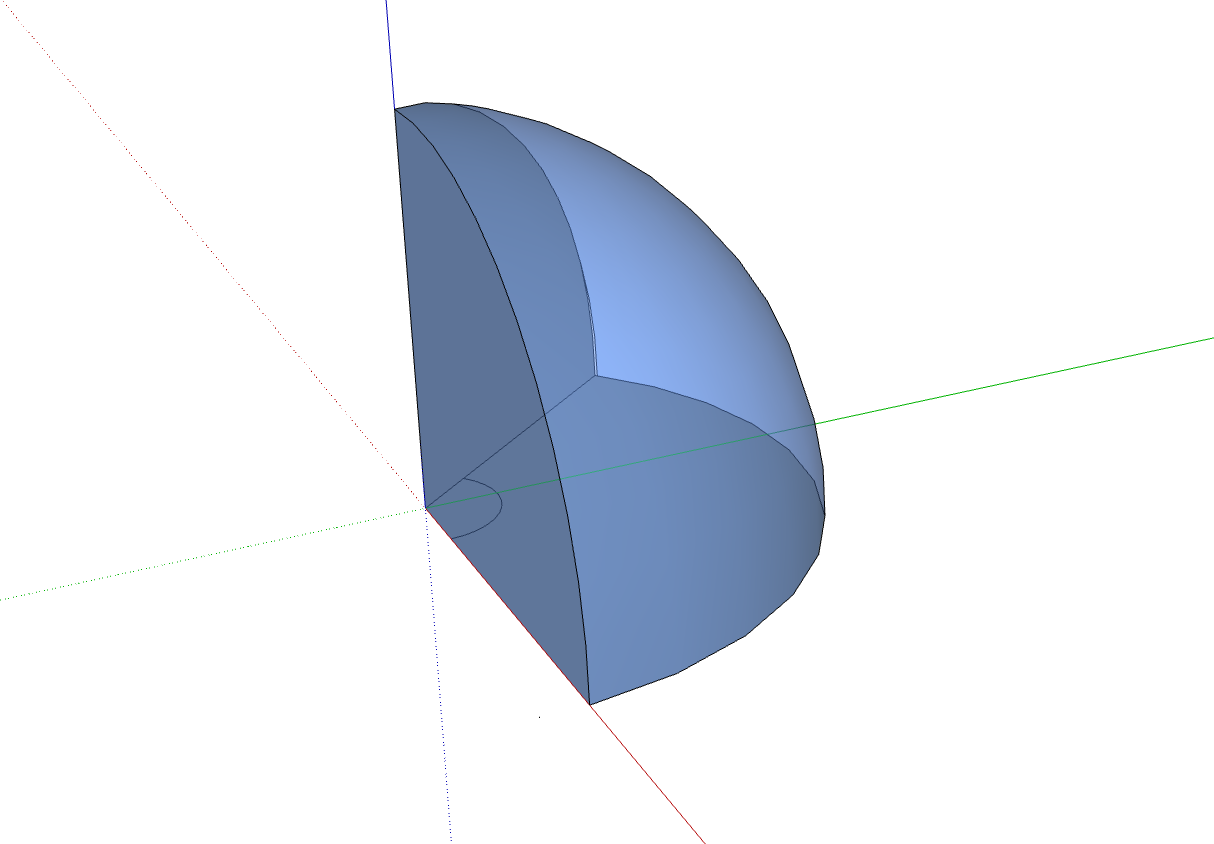
\includegraphics[width=15cm]{krhelj2.png}
    \caption{Krhelj.}
    \label{fig:krhelj}
\end{figure}
Na tem območju rešujemo difuzijsko enačbo brez izvorov

\begin{equation}
\frac{\partial T}{\partial t} = -D \nabla^2 T.
\end{equation}
Z nastavkom $ T(\vect{ r}, t) = u(\vect{ r})\tau (t)$ ločimo časovni del od krajevnega in dobimo

\begin{equation}
\frac{\tau '}{\tau} = - D \frac{\nabla^2 u}{u} = \lambda^2,
\end{equation}
kjer je $\lambda^2 >0$.
Rešitve časovnega dela so eksponentne funkcije, ker pa nas zanima temperatura za $t>0$, bo rešitev oblike

\begin{equation}
\tau (t) = A \mathrm{e} ^{-\lambda t}.
\end{equation}
Za krajevni del dobimo Helmhotzevo enačbo.
Sferično geometrijo upoštevamo v operatorju $\nabla ^2$, torej

\begin{equation}
\frac{1}{r^2} \frac{\partial}{\partial r}(r^2 \frac{\partial u}{\partial r}) - \frac{L^2 u}{r} + \gamma u = 0,
\label{eq:helmhotz}
\end{equation}
kjer je $\gamma = \lambda^2/D > 0$ in 

\begin{equation}
L^2 = - \frac{1}{\sin^2 \theta } \frac{\partial}{\partial \theta}(\sin \theta \frac{\partial }{\partial \theta}) - \frac{1}{\sin^2 \theta} \frac{\partial^2}{\partial \phi^2}.
\end{equation}
Lastne vrednosti in funkcije tega operatorja rešujemo s separacijo spremenljivk v obliki $u(\vect r) = R(r) \, \Theta (\theta) \, \Phi (\phi)$.
Ker $L^2$ deluje le na kotni del, lahko za ta namen izpustimo radialni del in zapišemo

\begin{equation}
L^2 \: \Theta (\theta) \Phi (\phi) = \Tilde \lambda \; \Theta (\theta) \Phi (\phi).
\end{equation}
Ločimo spremenljivke in dobimo enačbi

\begin{equation}
\frac{1-\cos^2\theta}{\Theta}\frac{\partial}{\sin \theta \: \partial \theta} \Big[ (1-\cos^2\theta)\frac{\partial}{\sin\theta \: \partial \theta} \Big ] \Theta + \tilde \lambda \;
=\; -\frac {1}{\Phi} \frac{\partial^2 \Phi}{\partial \phi^2} \;
=\; \mu^2.
\label{eq:L2}
\end{equation}
Rešimo najprej kotni del v smeri $\phi$:

\begin{equation}
\Phi(\phi) = C_\mu \sin (\mu \phi) + D_\mu \cos (\mu \phi).
\end{equation}
Dirichletovi robni pogoji nam dajo $D=0$ in $\mu = \frac{3}{2}m; \; \, m = 1, 2, 3, ...$ , torej je rešitev

\begin{equation}
\Phi(\phi) = C_m \sin \big(3/2 m \phi\big)
\label{eq:phi}
\end{equation}
Ostane nam še kotni del v smeri $\theta$.
Z uvedbo nove spremenljivke $z=\cos\theta$ prepišemo enačbo \ref{eq:L2} in dobimo

\begin{equation}
\frac{\partial}{\partial z} \Big[ (1-z^2)\frac{\partial}{\partial z} \Big ] \Theta + \Big[\tilde \lambda - \frac{\mu^2}{1-z^2} \Big] \Theta = 0.
\end{equation}
Če definiramo $\tilde \lambda = \nu (\nu+1)$, v zadnjem izrazu prepoznamo Legendrovo diferencialno enačbo.
Rešitve za spremenljivko $z$ so pridruženi Legendrovi polinomi oziroma, če upoštevamo $z=\cos \theta$, je rešitev oblike

\begin{equation}
\Theta(\theta) =  A_{\nu, \mu, n} P_\nu^\mu(\cos \theta) + B_{\nu, \mu, n} Q_\nu^\mu(\cos \theta).
\label{eq:theta}
\end{equation}
Spomnimo se, da je $\mu = 3/2 m$ in izločimo funkcije, ki divergirajo na definicijskem območju.
Za celoštevilske $\mu$ (sode $m$) nam ostanejo $P_\nu^\mu$, za polcele $\mu$ (lihe $m$) pa $Q_\nu^\mu$:
\begin{align*}
m=1:&\quad Q_{3/2}^{3/2}, \: Q_{5/2}^{3/2}, \: Q_{7/2}^{3/2},\; ...\\
m=2:&\quad P_3^3, \; \; \;  P_4^3,\; \; \;  P_5^3,\; ...\\
m=3:&\quad Q_{9/2}^{9/2}, \: Q_{11/2}^{9/2},\: Q_{13/2}^{9/2},\; ...\\
m=4:&\quad P_6^6,\; \; \; P_7^6,\; \; \; P_8^6,\; ...\\
\vdots
\end{align*}
Rešitve morajo ustrezati še Dirichletovim robnim pogojem, pri čemer si pomagamo grafično.
Iz zgornjega nabora funkcij rišemo $P_\nu^\mu$ in $Q_\nu^\mu$ na robu definicijskega območja, v odvisnosti od $\nu$.
\begin{figure}[H]
    \centering
    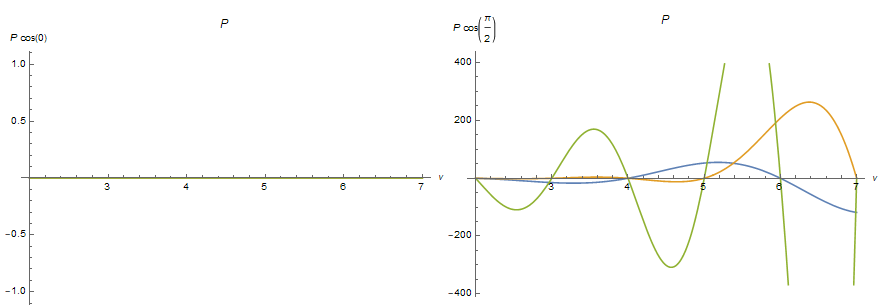
\includegraphics[width=16cm]{pnicle.png}
    \caption{$P_\nu^\mu(\cos 0)$ levo in $P_\nu^\mu(\cos 2\pi/3)$ desno, v odvisnosti od $\nu$, pri $\mu = 3, 6, 9$.}
    \label{fig:p}
\end{figure}

\begin{figure}[H]
    \centering
    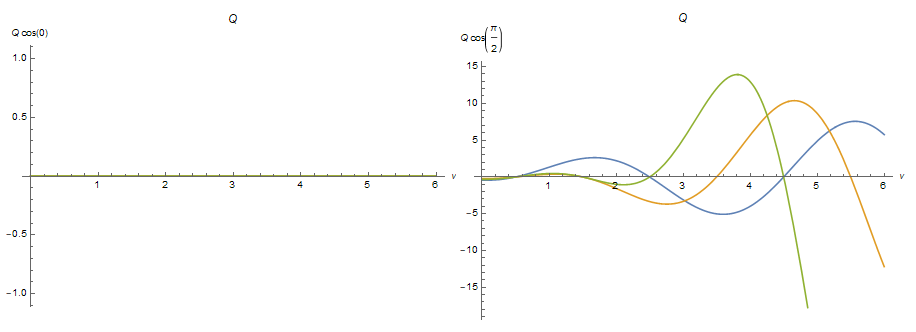
\includegraphics[width=16cm]{qnicle.png}
    \caption{$Q_\nu^\mu(\cos 0)$ levo in $Q_\nu^\mu(\cos 2\pi/3)$ desno, v odvisnosti od $\nu$, pri $\mu = 3/2, 9/2, 15/2$.}
    \label{fig:q}
\end{figure}
Ničle funkcij nam torej določajo dovoljene indekse $\nu$.
Iz slik (\ref{fig:p}) in (\ref{fig:q}) ugotovimo, da pri $\theta = 0$ robnemu pogoju zadoščajo vse zgoraj naštete funkcije, pri $\theta = \pi /2$ pa iz množice funkcij $P_\nu^\mu$ temu ustrezajo tiste, ki imajo sodo-lihe ali liho-sode indekse $\nu$ in $\mu$.
Podobna relacija velja za indekse funkcij $Q_\nu^\mu$, če jih premaknemo za $1/2$.
Ostane nam naslednji nabor funkcij:
\begin{align*}
m=&1:\quad Q_{3/2}^{5/2},\: Q_{9/2}^{3/2}, \: Q_{13/2}^{3/2},\; ...\\
m=&2:\quad P_4^3,\; \; \; P_6^3,\; \; \; P_8^3,\; ...\\
m=&3:\quad Q_{11/2}^{9/2}, \: Q_{15/2}^{9/2}, \: Q_{19/2}^{9/2},\; ...\\
m=&4:\quad P_7^6,\; \; \; P_9^6,\; \; \; P_{11}^6,\; ...\\
\vdots&
\end{align*}


Enačbi \ref{eq:phi} in \ref{eq:theta} vstavimo nazaj v \ref{eq:helmhotz} ter dobimo enačbo za radialni del

\begin{equation}
\frac{1}{r^2} \frac{\partial}{\partial r}\Big(r^2 \frac{\partial R}{\partial r}\Big) - \frac{\nu(\nu+1)}{r^2}R + \gamma R = 0.
\end{equation}
Ta izraz prepišemo z uvedbo nove spremenljivke $R(r)=\frac{S(r)}{\sqrt{r}}$:

\begin{equation}
r^2S'' + rS' + [\gamma r^2 - (\nu+\frac{1}{2})^2]S = 0.
\end{equation}
Dobili smo Besslovo diferencialno enačbo za funkcijo $S$.
Rešitve radialnega dela $R$ pa so sferične Besselove funkcije, izmed katerih zopet izločimo tiste, ki divergirajo v izhodišču.
Ostanejo nam sferični Bessli prve vrste, ki morajo zadoščati robnemu pogoju $R(R_0) = 0$.
Dobimo

\begin{equation}
R(r) = E_{\nu,n} \; \mathrm{j}_\nu \big(\zeta_{\nu, n} r/R_0\big),
\end{equation}
kjer je $\zeta_{\nu, n}$ $n$-ta ničla $\nu$-te sferične Besselove funkcije.

Končno rešitev zapišemo kot vsoto
\begin{equation}
T(\vect r, t) = \sum_{\nu, \mu, n} \Big[A_{\nu, \mu, n} P_\nu^\mu(\cos \theta) + B_{\nu, \mu, n} Q_\nu^\mu(\cos \theta) \Big]
	\sin(\mu \phi) \:
	\mathrm{j}_\nu \big(\zeta_{\nu, n} r/R_0\big) \:
	\mathrm{e}^{-\sqrt{D} \zeta_{\nu, n}/R_0 t},
\label{eq:splosna}
\end{equation}
pri čemer upoštevamo, da je $\mu = 3/2m$ in $m$ teče po naravnih številih.

\vspace{0.5cm}









\section{Lega maksimalne temperature}


Za maksimum temperature moramo rešiti enačbo $\nabla T(\vect r, t) = \vect 0$, ki jo v sferičnih koordinatah zapišemo kot

\begin{equation}
\begin{bmatrix}
\frac{\partial}{\partial r} \\
\frac{1}{r}\frac{\partial}{\partial \theta} \\
\frac{1}{r \sin \theta}\frac{\partial}{\partial \phi}
\end{bmatrix}
 T(\vect r, t) = \vect 0.
\end{equation}
Če jo rešujemo po komponentah, dobimo sistem enačb za $r(t)$, $\theta(t)$ in $\phi(t)$

\begin{equation}
\begin{split}
\sum_{\nu, \mu, n}  \Big[A_{\nu, \mu, n} P_\nu^\mu(\cos \theta) + B_{\nu, \mu, n} Q_\nu^\mu(\cos \theta) \Big]
	\sin(\mu \phi)\frac{\partial}{\partial r} \mathrm{j}_\nu \big(\zeta_{\nu, n} r/R_0\big)
	\mathrm{e}^{-\sqrt{D} \zeta_{\nu, n}/R_0 t} = 0, \\
\sum_{\nu, \mu, n} \frac{\partial}{\partial \theta} \Big[A_{\nu, \mu, n} P_\nu^\mu(\cos \theta) + B_{\nu, \mu, n} Q_\nu^\mu(\cos \theta) \Big]
	\sin(\mu \phi) \frac{ \mathrm{j}_\nu \big(\zeta_{\nu, n} r/R_0\big)}{r}
	\mathrm{e}^{-\sqrt{D} \zeta_{\nu, n}/R_0 t} = 0, \\
\sum_{\nu, \mu, n} \frac{A_{\nu, \mu, n} P_\nu^\mu(\cos \theta) + B_{\nu, \mu, n} Q_\nu^\mu(\cos \theta)}{\sin \theta}
	\mu \cos(\mu \phi) \frac{\mathrm{j}_\nu \big(\zeta_{\nu, n} r/R_0\big)}{r}
	\mathrm{e}^{-\sqrt{D} \zeta_{\nu, n}/R_0 t} = 0,
\end{split}
\end{equation}
ki, razen v posebnih primerih, ni analitično rešljiv, zato se poslužimo numeričnih približkov.







\subsection{Konstantna začetna temperatura}


Najprej nas zanima rešitev za začetni pogoj $T(\vect r, 0) = T_0$.
Izrazimo ga z enačbo \ref{eq:splosna}, skalarno pomnožimo z drugo funkcijo iz baze in upoštevamo ortogonalnost

\begin{equation}
\begin{split}
T_0\int \sum \Big[A_{\nu', \mu', n'} P_{\nu'}^{\mu'}(\cos \theta) + B_{\nu', \mu', n'} Q_{\nu'}^{\mu'}(\cos \theta) \Big]
	\sin(\mu' \phi) \mathrm{j}_{\nu'} \big(\zeta_{\nu', n'} r/R_0\big) \dd ^3 \vect r = \\	
	 = \int \sum \Big[A_{\nu', \mu', n'}^2 P_{\nu'}^{\mu' \, 2}(\cos \theta) + B_{\nu', \mu', n'}^2 Q_{\nu'}^{\mu' \, 2}(\cos \theta) \Big]
	\sin^2(\mu' \phi) \mathrm{j}_{\nu'}^2 \big(\zeta_{\nu', n'} r/R_0\big) \dd ^3 \vect r
\end{split}
\end{equation}
Ker v posameznih členih vsote po $m$ nastopa bodisi $P_{\nu'}^{\mu'}$ bodisi $Q_{\nu'}^{\mu'}$, lahko ločimo primera za sode in lihe $m$ ter izrazimo konstanti $A_{\nu, \mu, n}$ in $B_{\nu, \mu, n}$

\begin{equation}
\begin{split}
A_{\nu, \mu, n} &= \frac{2\frac{1-(-1)^m}{m} \int_1^0 P_{\nu}^{\mu}(z) \dd z\int_0^1 r^2 \mathrm{j}_\nu (\zeta_{\nu,n} r) \dd r}
	{\pi  \int_1^0 P_{\nu}^{\mu \, 2}(z) \dd z\int_0^1 r^2 \mathrm{j}_\nu^2 (\zeta_{\nu,n} r) \dd r}T_0 =0  \ \ ; \quad m \text{ sod}, \\
B_{\nu, \mu, n} &= \frac{2\frac{2}{m} \int_1^0 Q_{\nu}^{\mu}(z) \dd z\int_0^1 r^2 \mathrm{j}_\nu (\zeta_{\nu,n} r) \dd r}
	{\pi  \int_1^0 Q_{\nu}^{\mu \, 2}(z) \dd z\int_0^1 r^2 \mathrm{j}_\nu^2 (\zeta_{\nu,n} r) \dd r}T_0 \ \ ; \hspace{15mm} \quad m \text{ lih}.
\end{split}
\end{equation}
Integral po polarnem kotu izloči vse člene s $P_{\nu}^\mu$ in ostane

\begin{equation}
T(\vect r, t) = \sum_{\nu, \mu, n}  B_{\nu, \mu, n} Q_\nu^\mu(\cos \theta)
	\sin(\mu \phi) \mathrm{j}_\nu \big(\zeta_{\nu, n} r/R_0\big)
	\mathrm{e}^{-\sqrt{D} \zeta_{\nu, n}/R_0 t}.
\end{equation}
Iz simetrije problema v smeri $\phi$ lahko uganemo, da se bo maksimalna temperatura vseskozi nahajala pri $\phi = \pi/3$.
$r(t)$ in $\theta(t)$ za maksimum poiščemo numerično.

\begin{figure}[H]
    \centering
    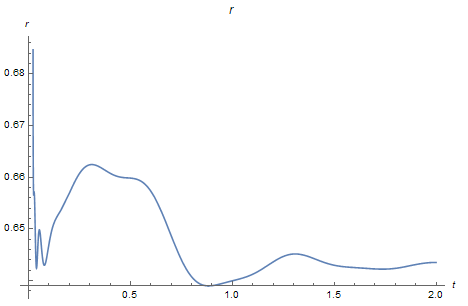
\includegraphics[width=8cm]{1r.png}
    \caption{$r(t)$ pri katerem je maksimum $T$.}
    \label{fig:pq}
\end{figure}
\begin{figure}[H]
    \centering
    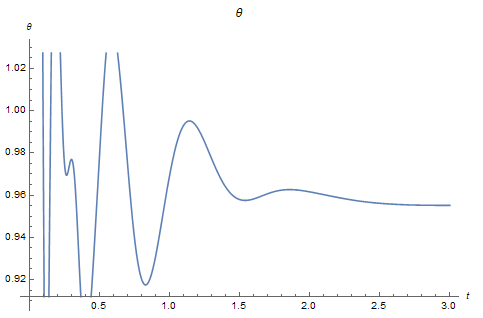
\includegraphics[width=8cm]{theta1.png}
    \caption{$\theta(t)$ pri katerem je maksimum $T$.}
    \label{fig:pq}
\end{figure}




\subsection{Temperatura narašča z azimutalnim kotom}

Začetni pogoj zapišemo v obliki $T(\vect r, 0) = \alpha \phi$.
V tem primeru dobimo tudi člene s $P_{\nu}^{\mu}$.
Po enakem postopku, kot v prejšnjem razdelku pridelamo koeficiente $A$ in $B$.
Tokrat je integral po kotu $\phi$, ki določa konstanti $A$ in $B$, enak $-\frac{4 \pi \alpha}{9}\frac{(-1)^m}{m}$ in od tod

\begin{equation}
\begin{split}
A_{\nu, \mu, n} &= \frac{2 \: \big(- \frac{4 \pi \alpha}{9 m} \big) \int_1^0 P_{\nu}^{\mu}(z) \dd z\int_0^1 r^2 \mathrm{j}_\nu (\zeta_{\nu,n} r) \dd r}
	{\pi  \int_1^0 P_{\nu}^{\mu \, 2}(z) \dd z\int_0^1 r^2 \mathrm{j}_\nu^2 (\zeta_{\nu,n} r) \dd r}T_0 \ \ ; \quad m \text{ sod}, \\
B_{\nu, \mu, n} &= \frac{2 \: \frac{4 \pi \alpha}{9 m} \int_1^0 Q_{\nu}^{\mu}(z) \dd z\int_0^1 r^2 \mathrm{j}_\nu (\zeta_{\nu,n} r) \dd r}
	{\pi  \int_1^0 Q_{\nu}^{\mu \, 2}(z) \dd z\int_0^1 r^2 \mathrm{j}_\nu^2 (\zeta_{\nu,n} r) \dd r}T_0 \ \ ; \hspace{8mm} \quad m \text{ lih}.
\end{split}
\end{equation}
$r(t)$, $\theta(t)$ in $\phi(t)$ za maksimum zopet poiščemo numerično.

\begin{figure}[H]
    \centering
    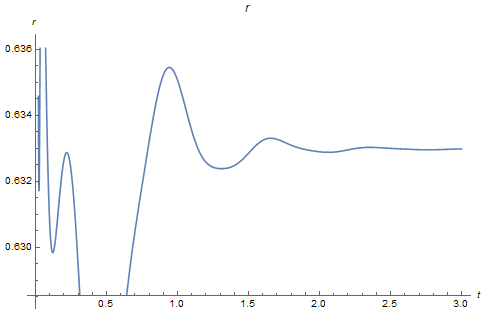
\includegraphics[width=8cm]{2r.png}
    \caption{$r(t)$ pri katerem je maksimum $T$}
    \label{fig:pq}
\end{figure}
\begin{figure}[H]
    \centering
    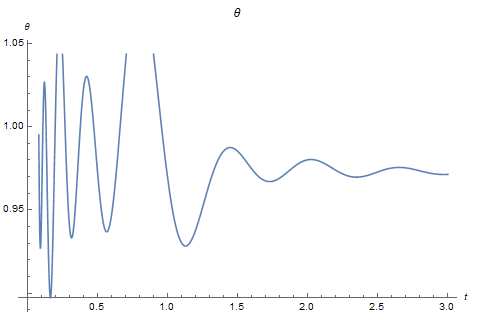
\includegraphics[width=8cm]{theta2.png}
    \caption{$\theta(t)$ pri katerem je maksimum $T$.}
    \label{fig:pq}
\end{figure}
\begin{figure}[H]
    \centering
    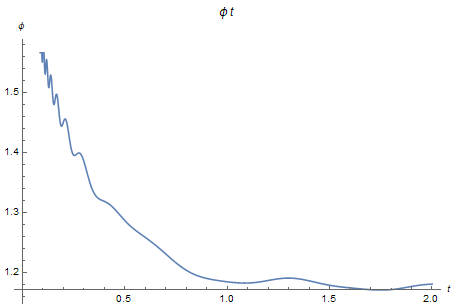
\includegraphics[width=8cm]{2phi2.png}
    \caption{$\phi(t)$ pri katerem je maksimum $T$.}
    \label{fig:pq}
\end{figure}

V obeh primerih je vrednost $r$ skalirana na $r/R_0$, $\theta$ in $\phi$ pa v radianih.
Če izračunamo težišče krhlja, dobimo
\begin{equation}
\vect {r}_T=
\begin{bmatrix}
\frac{3\sqrt{43}}{32} \\
\arccos (\frac{4}{\sqrt{43}}) \\
\pi/3
\end{bmatrix}
\approx
\begin{bmatrix}
0,614 \\
0,915 \\
1,047
\end{bmatrix},
\end{equation}
kar se približno ujema z vrednostmi v limiti za velike čase.
Za majhne čase je numerični približek neuporaben oziroma, za dobro aproksimacijo zahteva bistveno večje število členov v vsotah.


\end{document}